\documentclass[12pt, a4paper, oneside, UTF8]{ctexart}
\usepackage{amsmath, amsthm, amssymb, bm, color, framed, graphicx, hyperref, mathrsfs}
\usepackage{geometry}
\geometry{left = 2.5 cm, right = 2.5 cm, top = 2.5 cm, bottom = 2.5 cm}

\title{\textbf{作业9}\\{\small (数值算法与案例分析)}}
\author{李维杰}
\date{\today}
\linespread{1.5}
\definecolor{shadecolor}{RGB}{241, 241, 255}
\newcounter{problemname}
\newenvironment{problem}{\begin{shaded}\stepcounter{problemname}\par\noindent\textbf{题目\arabic{problemname}. }}{\end{shaded}\par}
\newenvironment{solution}{\par\noindent\textbf{解答. }}{\par}
\newenvironment{note}{\par\noindent\textbf{注记. }}{\par}

\newcommand{\pll}{\kern 0.56em/\kern -0.8em /\kern 0.56em}

\begin{document}

\maketitle

\begin{problem}
    设$\hat{x} \in \mathbb{R}^{n}$是实对称矩阵$A$的一个近似特征向量,且满足${\left\lVert{\hat{x}}\right\rVert}_{2}=1$.证明:存在一个实对称矩阵$\Delta A$,使得
    \begin{align*}
        (A + \Delta A)\hat{x} = \hat{x} \hat{\lambda},&&{\left\lVert{\Delta A}\right\rVert}_{2} \leq {\left\lVert{A\hat{x} - \hat{x}\hat{\lambda}}\right\rVert}_{2}
    \end{align*}
    成立,其中$\hat{\lambda} = \hat{x}^{T} A \hat{x}$.
\end{problem}

\begin{solution}
    对$(A + \Delta A)\hat{x} = \hat{x} \hat{\lambda}$两边同时左乘$\hat{x}^T$,可得此式的一个必要条件
    \begin{align*}
        \hat{x}^T \Delta A \hat{x} = 0,
    \end{align*}
    也即$\Delta A \hat{x} \bot \hat{x}$.又由于
    \begin{align*}
        \hat{x}^T (\hat{x}\hat{\lambda} - A\hat{x}) = 0,
    \end{align*}
    即$\hat{x}\hat{\lambda}-A\hat{x} \bot \hat{x}$, 故$\hat{x}\hat{\lambda}-A\hat{x} \pll \Delta A \hat{x}$.
    定义Householder镜射向量
    \begin{align*}
        v=\frac{1}{\sqrt{2}}({\hat{x}-\frac{\hat{x} \hat{\lambda} - A \hat{x}}{\left\lVert{\hat{x} \hat{\lambda} - A \hat{x}}\right\rVert}_{2}}),
    \end{align*}
    则$\Delta A = k(I - 2vv^T)$是符合要求的一个必要条件,其中$k$是常数.事实上,当$k={\left\lVert{\hat{x} \hat{\lambda} - A \hat{x}}\right\rVert}_{2}$时,有
    \begin{align*}
        (A + \Delta A)\hat{x} = A \hat{x} + {\left\lVert{\hat{x} \hat{\lambda} - A \hat{x}}\right\rVert}_{2}\hat{x} - [({\left\lVert{\hat{x} \hat{\lambda} - A \hat{x}}\right\rVert}_{2}-\hat{\lambda})I+A]\hat{x}=\hat{x}\hat{\lambda},
    \end{align*}
    且
    \begin{align*}
        {\left\lVert{\Delta A}\right\rVert}_{2} = {\left\lVert{\hat{x} \hat{\lambda} - A \hat{x}}\right\rVert}_{2}{\left\lVert{I - 2 v v^T}\right\rVert}_{2} = {\left\lVert{\hat{x} \hat{\lambda} - A \hat{x}}\right\rVert}_{2}.
    \end{align*}
    于是此时的$\Delta A$即为一个符合题意的构造.
\end{solution}

\begin{problem}
    给定$x,y \in \mathbb{R}^{n}$.详细描述如何构建一个旋转矩阵$Q$,使得$\left[\begin{array}{cc}x & y\end{array}\right]Q$的列向量是相互正交的.
\end{problem}

\begin{solution}
    设$Q=\left[
        \begin{array}{cc}	
            \cos{\theta} & \sin{\theta} \\
            -\sin{\theta} & \cos{\theta}
        \end{array}
    \right]$,则在旋转作用后,相应元素变换为
    \begin{align*}
        \left\{
            \begin{array}{ll}
                x_i \leftarrow x_i \cos{\theta} - y_i \sin{\theta} \\
                y_i \leftarrow x_i \sin{\theta} + y_i \cos{\theta}
            \end{array}
        \right. ,
    \end{align*}
    我们希望变换后满足$x^T y = 0$, 也即
    \begin{align*}
        x^T y &= \sum\limits_{i=1}^{n}{x_i y_i} \\
        &= \sum\limits_{i=1}^{n}{(x_{i}^{2} \cos{\theta} \sin{\theta} - y_{i}^{2} \cos{\theta} \sin{\theta} +x_i y_i (\cos^2{\theta} - \sin^2{\theta}))} \\
        &= ({\left\lVert{x}\right\rVert}_{2}^{2} - {\left\lVert{y}\right\rVert}_{2}^{2})\cos{\theta}\sin{\theta} + x^T y (\cos^2{\theta} - \sin^2{\theta}) \\
        &= 0 .
    \end{align*}
    进一步整理成方程
    \begin{align*}
        x^T y \tan^2{\theta} - ({\left\lVert{x}\right\rVert}_{2}^{2} - {\left\lVert{y}\right\rVert}_{2}^{2})\tan{\theta} - x^T y = 0 .
    \end{align*}
    解上述关于$\tan{\theta}$的一元二次方程即可得满足题意的旋转矩阵$Q$.
\end{solution}

\begin{problem}
    设$D \in \mathbb{R}^{n \times n}$是具有不同特征值的对角阵, $z \in \mathbb{R}^{n}$是一个没有零元素的向量,以及$\rho \in \mathbb{R} \backslash \{0\}$.
    假设$(\lambda, u)$是$D+\rho z z^T$的一个特征对,证明:\\
    (1) $\lambda I - D$是非奇异的;\\
    (2) $(\lambda I - D)^{-1}z$是$D + \rho z z^T$的一个特征向量;\\
    (3) $z^T u \neq 0$.
\end{problem}

\begin{solution}
    (1) 由于$(\lambda,u)$是$D + \rho z z^T$的一个特征对,故$D u + \rho z z^T u = \lambda u$, 进而有
    \begin{align*}
        (\lambda I - D) u = \rho z z^T u = (\rho z^T u) z,
    \end{align*}
    即对角阵$(\lambda I - D)$将$u$映射到不包含零元素的向量$z$的方向上,故$(\lambda I - D)$是非奇异的.\\
    (2) 对于$(D + \rho z z^T)$, 由于特征多项式
    \begin{align*}
        f(\lambda) = (1 - \rho z^T (D - \lambda I)^{-1} z)\det{D} = 0 \Rightarrow (\rho z^T (\lambda I - D)^{-1} z) - 1 = 0.
    \end{align*}
    于是有
    \begin{align*}
        (D + \rho z z^T)(\lambda I - D)^{-1}z &= -z + \lambda(\lambda I - D)^{-1}z + \rho z^T(\lambda I - D)^{-1} z z \\
        &= [\rho z^T (\lambda I - D)^{-1} z -1]z + \lambda(\lambda I - D)^{-1} z \\
        &= \lambda(\lambda I - D)^{-1} z,
    \end{align*}
    也即$(\lambda, (\lambda I - D)^{-1}z)$是$D + \rho z z^T$的一个特征对. \\
    (3) 由(2)知$u = (\lambda I - D)^{-1}z$, 以及
    \begin{align*}
        (\rho z^T (\lambda I - D)^{-1} z) - 1 = 0 \Rightarrow z^T (\lambda I - D)^{-1} z = \frac{1}{\rho} \neq 0.
    \end{align*}
\end{solution}

\begin{problem}
    随机生成一个线性相关的小规模实对称矩阵$A = \text{diag}\{d_1,d_2,...,d_n\} + z z^T$, 其中$d_i$互不相同, 且$z$不含有零元素.
    可视化函数$$f(\lambda) = 1 - \sum\limits_{i=1}^{n}{\frac{z_i^2}{{\lambda - d_i}}}.$$
    同时在plot中突出显示$A$的特征值,确保它们与$f(\lambda)$的零点相匹配.为了简化问题, 你可以使用已有的函数库来计算$A$的特征值.
\end{problem}

\begin{solution}
    (代码见Problem4.m)
    \begin{figure}[htbp]
        \centering
        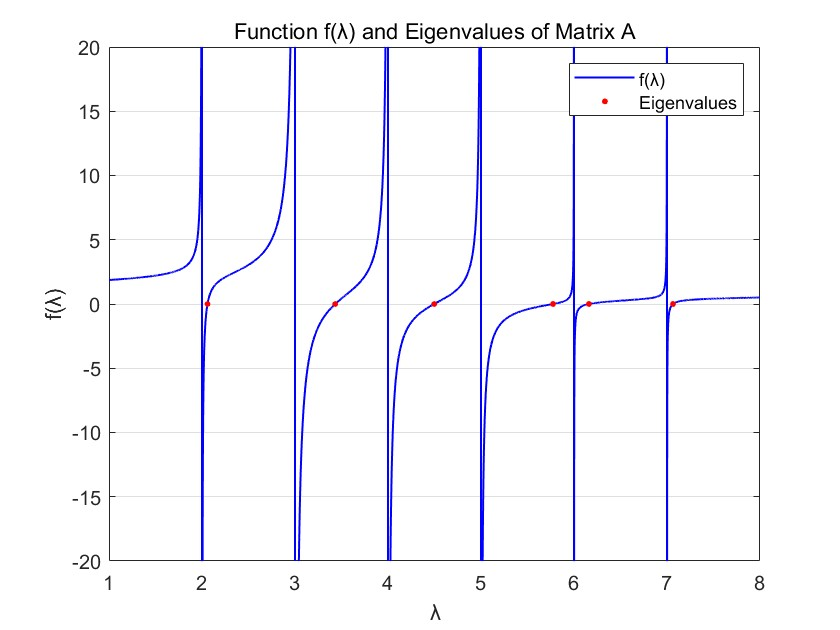
\includegraphics[scale=0.4]{Problem4.jpg}
        \caption{$f(\lambda)$图像与$\lambda$分布的关系图}
    \end{figure}
\end{solution}

\begin{problem}
    对实对称矩阵运用Jacobi对角化算法.可视化算法对一些规模不同的矩阵的表现. 同时可视化一个例子的收敛历程.\\
    鼓励可视化分量收敛结果和尝试选择错误Jacobi旋转矩阵(即不选最大元进行操作)的循环Jacobi算法.
\end{problem}
    
\begin{solution}
    (代码见Problem5(1).m)
    \begin{figure}[htbp]
        \centering
        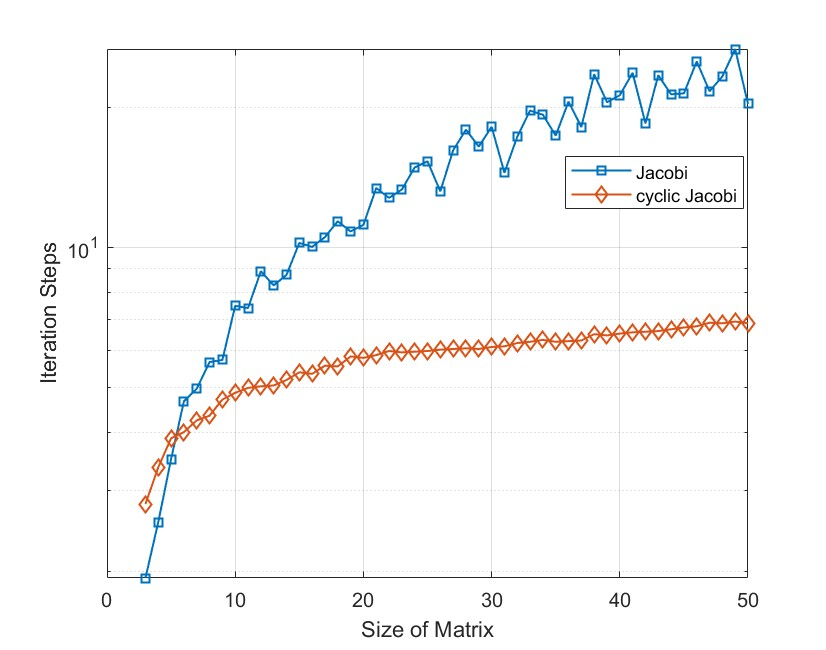
\includegraphics[scale=0.3]{Problem5-1.jpg}
        \caption{两类Jacobi算法的迭代表现}
    \end{figure} \\
    (代码见Problem5(2).m,其中刻画矩阵与对角阵的距离的量为${\left\lVert{A - Diag(A)}\right\rVert}_{\mathsf{F}}$)
    \begin{figure}[htbp]
        \centering
        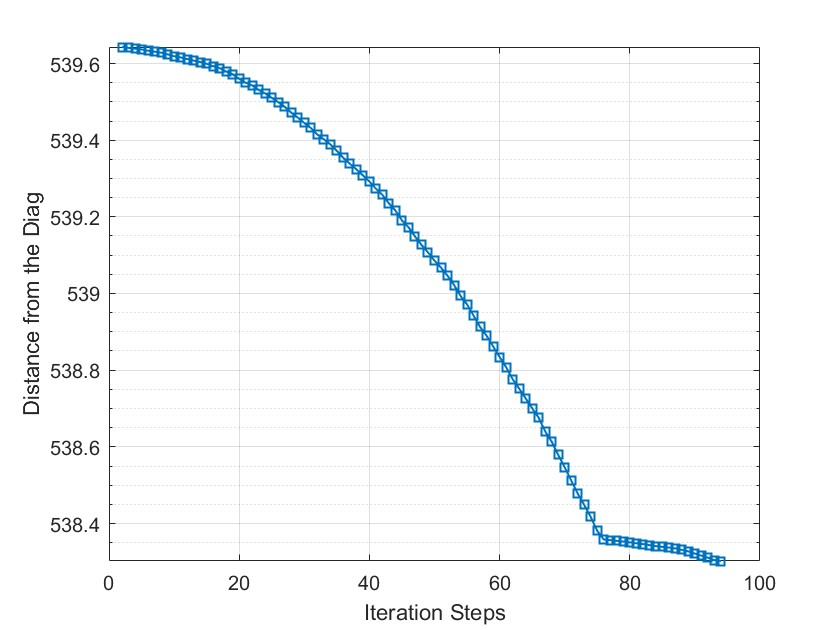
\includegraphics[scale=0.3]{Problem5-2.jpg}
        \caption{Jacobi算法对$1000 \times 1000$矩阵迭代的收敛历程}
    \end{figure}
\end{solution}

\end{document}